\chapter{シミュレーション結果}
\section{DCポテンシャル}
\Eq{rectangle_electrode}より,dc電圧を計算するためには電極モデルを矩形の形に分割する必要がある.Mathematica上における電極の分割の様子を\Fig{rect_electrode}に示す.
\begin{figure}[h]
	\begin{center}
		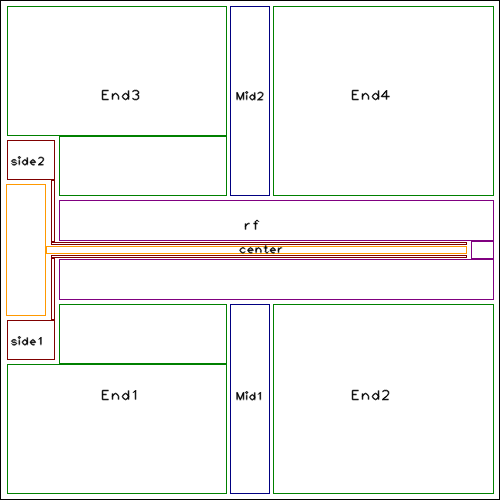
\includegraphics[width = 0.4\linewidth]{./simulation/figure/named_rect_electrode.png}
	\end{center}
	\caption{a}
	\label{fig:rect_electrode}
\end{figure}
各dc電極によってプレーナートラップ上の点$(x,y,z)$に形成される静電ポテンシャル$\Phi_{\rm DC}(x,y,z)$は,分割した各矩形が$(x,y,z)$に形成する静電ポテンシャルの重ね合わせで
\large
\begin{align}
	\Phi_{\rm DC}(x,y,z) = \phi_{\rm End1} + \phi_{\rm End2} + \phi_{\rm End3} &+ \phi_{\rm End4} + \phi_{\rm Mid1} + \phi_{\rm Mid2} \notag \\
	&+ \phi_{\rm Side1} + \phi_{\rm Side2} + \phi_{\rm center},
\end{align}
\normalsize
と表すことができる.
\begin{figure}[h]
	\begin{center}
		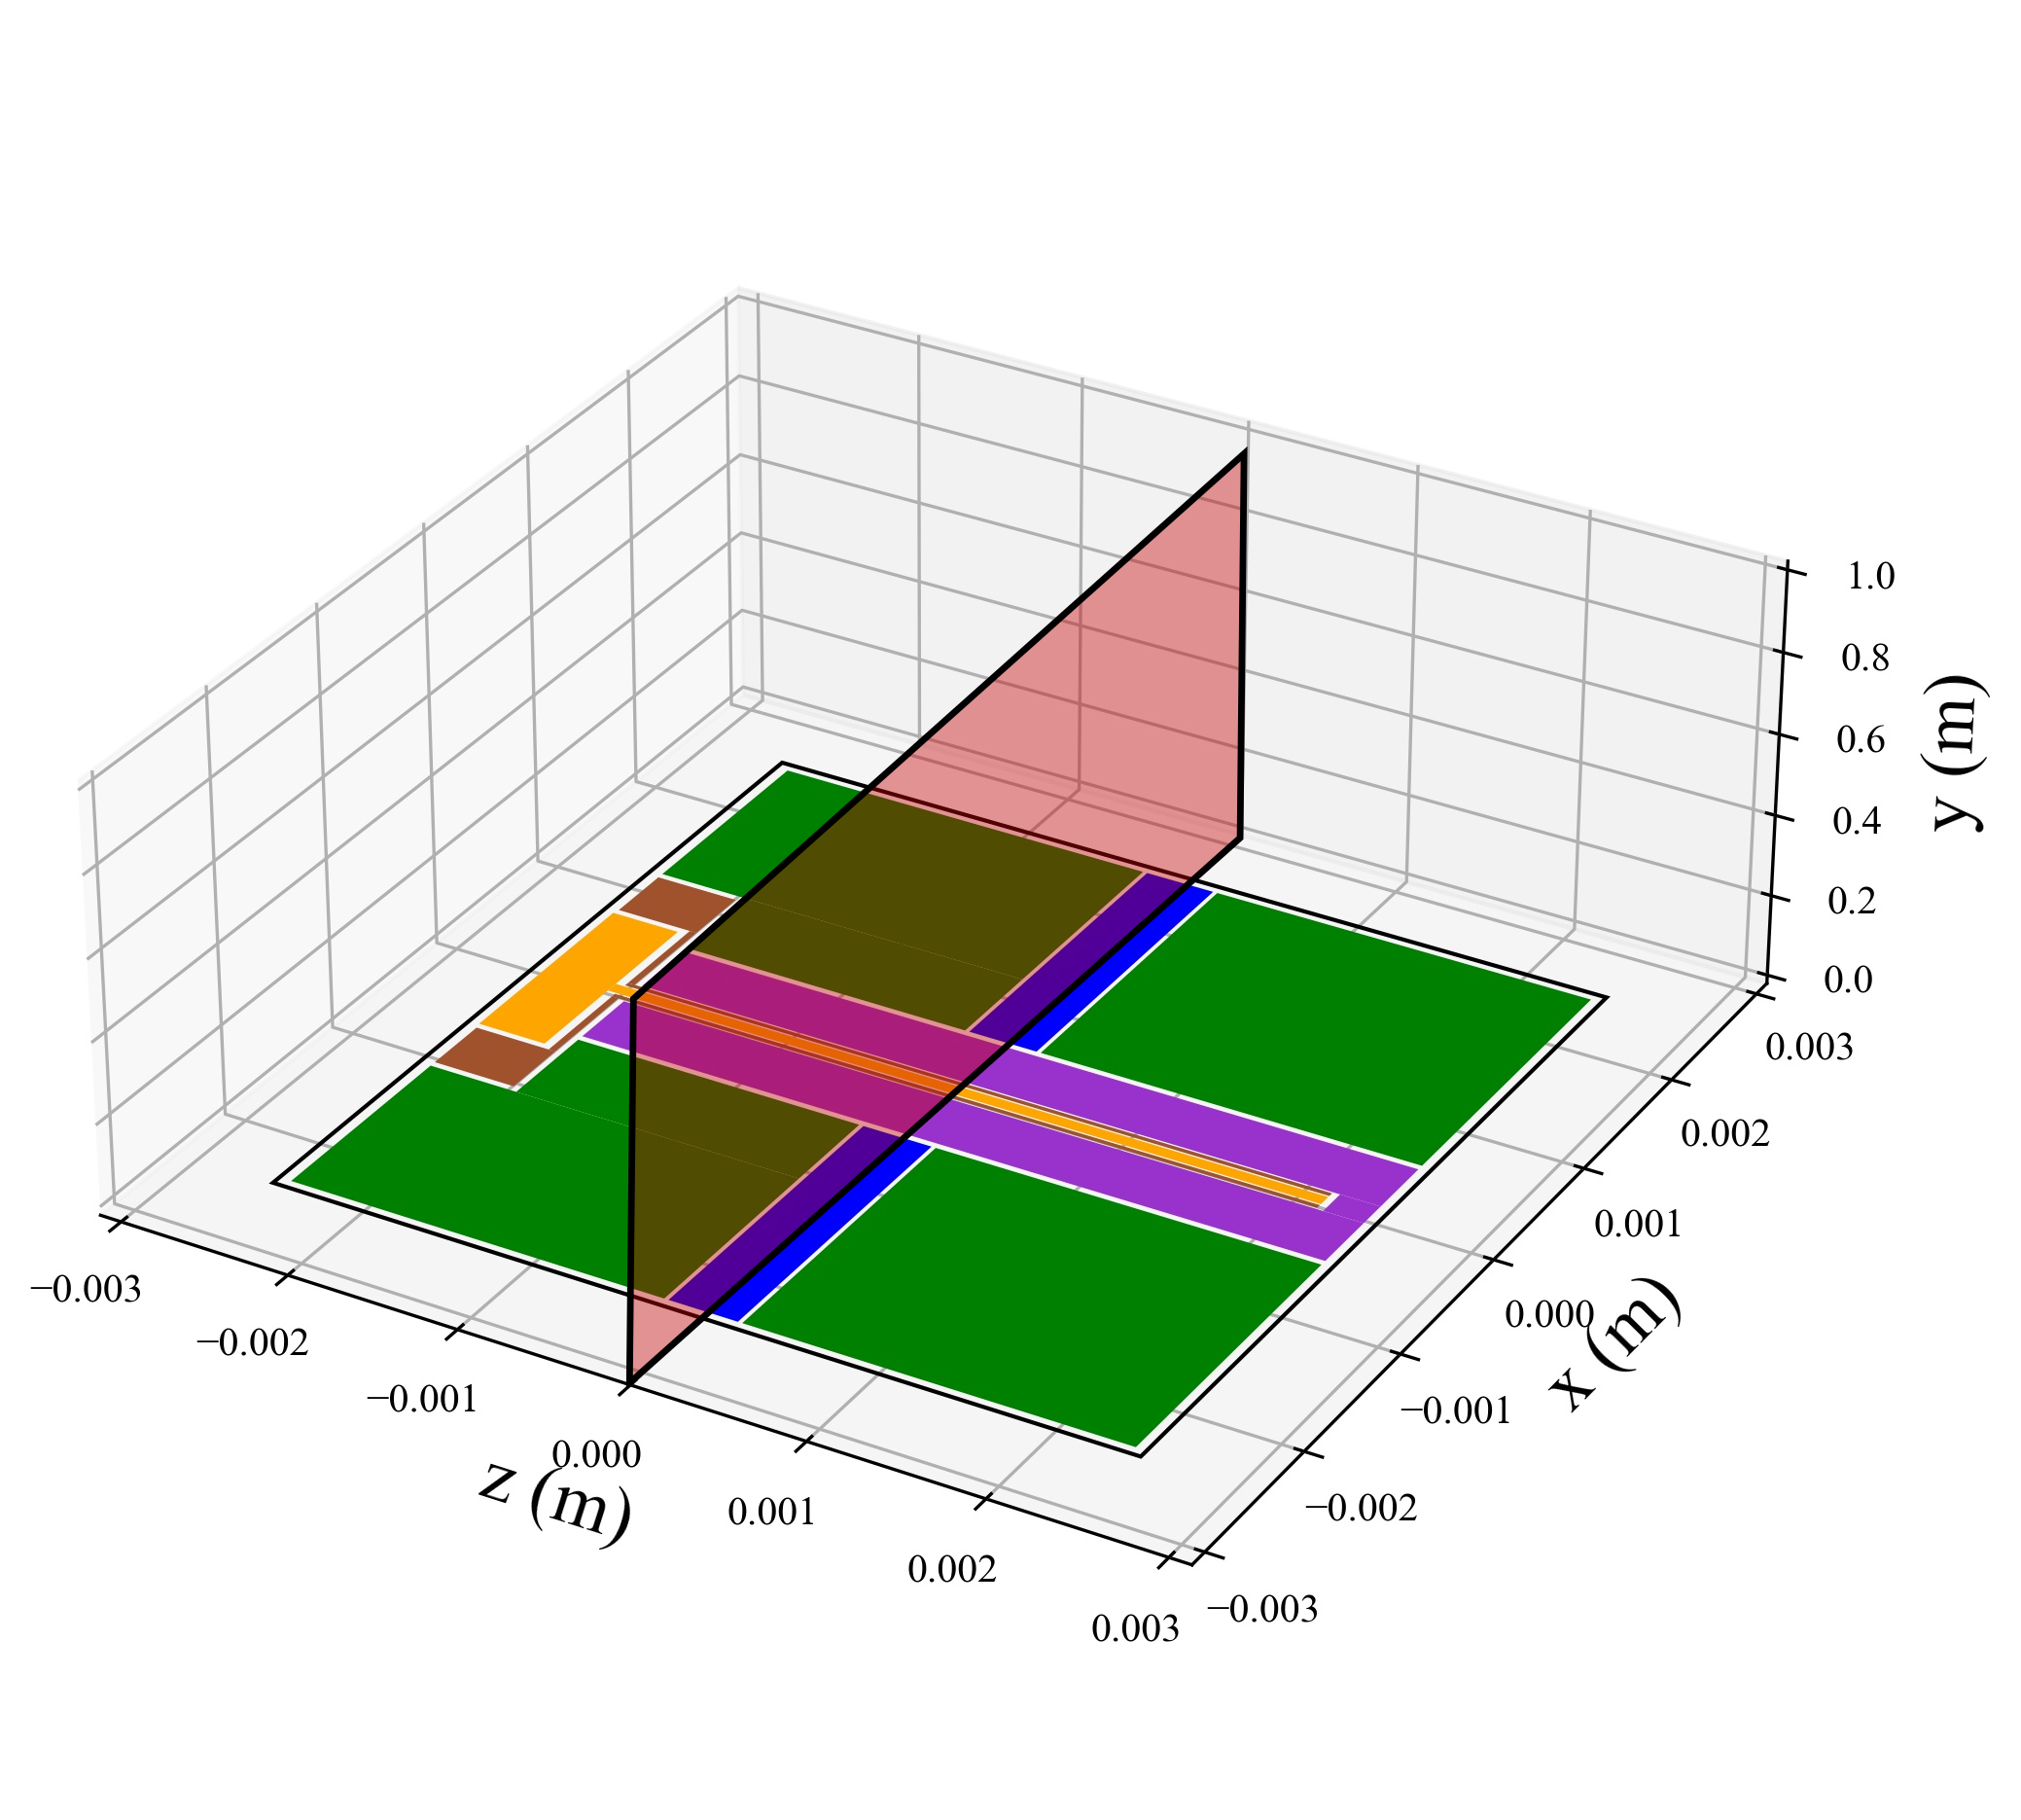
\includegraphics[width = 0.7\linewidth]{./simulation/figure/PlannarTrap_3D_z=0.png}
		\caption{プレーナートラップ上におけるz-y平面(x=0)}
	\end{center}
\end{figure}
\begin{figure}[h]
	\begin{center}
		\begin{minipage}{0.45\linewidth}
			\begin{center}
				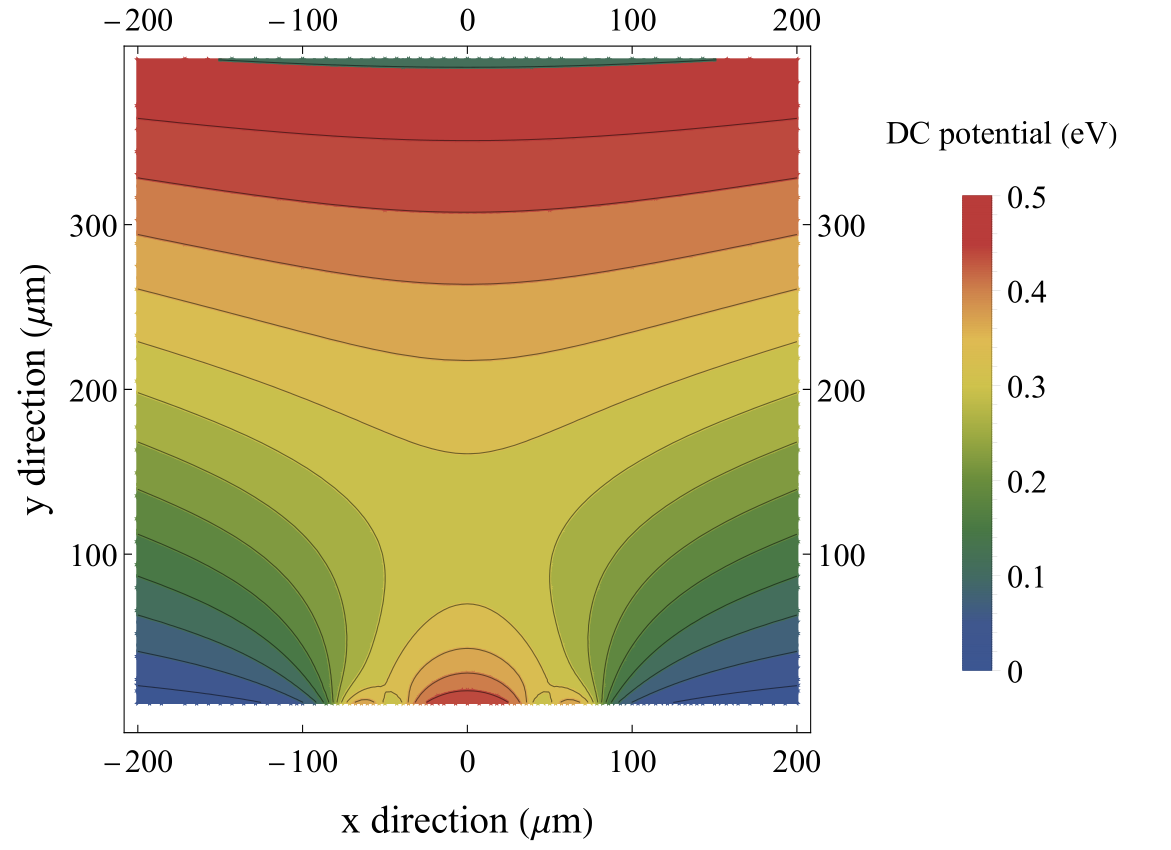
\includegraphics[width = 0.9\columnwidth]{./simulation/figure/dc_potential_example.png}
					\caption{z-y平面(x=0)での\Tb{dc_set1}の条件で計算したdcポテンシャル}
			\end{center}
		\end{minipage}
		\begin{minipage}{0.45\linewidth}
			\begin{center}
				\caption{dc電圧セット ${\rm DC}_{1}$}
				\label{tab:dc_set1}
				\begin{tabular}{c|c} \hline \hline
					電極 & 印加電圧 ()V) \\ \hline
					End1 & 1.41 \\ \hline
					End2 & 1.41 \\ \hline
					End3 & 1.41 \\ \hline
					End4 & 1.41 \\ \hline
					Mid1 & -1.532 \\ \hline
					Mid2 & -1.532 \\ \hline
					Side1 & 0.222 \\ \hline
					Side2 & 0.222 \\ \hline
					center & 0.225 \\ \hline
				\end{tabular}
			\end{center}
		\end{minipage}
	\end{center}
\end{figure}

\clearpage

\section{Single-wellにおけるrf擬ポテンシャル}
Single-wellの条件でのrf擬ポテンシャルについての計算結果を示す.\Fig{single-well_example_xy}にx-y平面(z=0)のrf擬ポテンシャルの計算結果を示す.このとき$\Omega_{\rm rf} = 27.2 \ {\rm MHz}, V_{\rm rf} = 62 \ V,R = 0.27$とした.
\begin{figure}[h]
	\begin{center}
	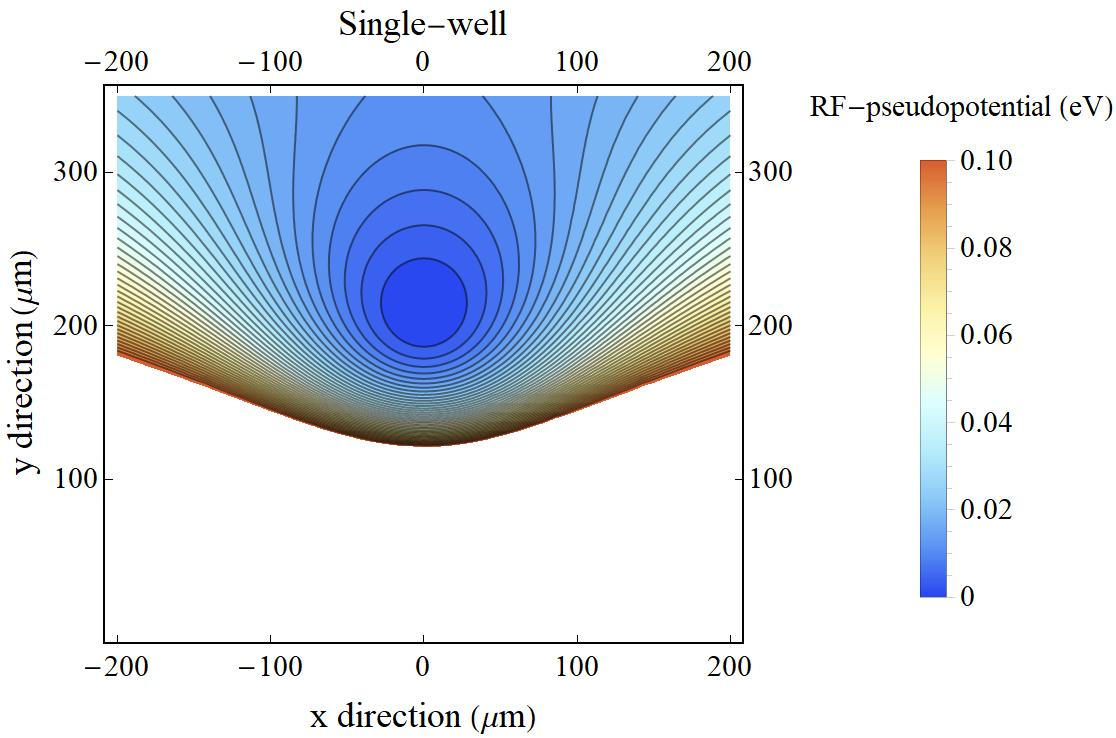
\includegraphics[width = 0.7\linewidth]{./simulation/figure/Single-well_Contour_xy@z=0.jpg}
	\caption{x-y平面(x=0)でのSingle-wellにおけるrf擬ポテンシャル}
	\label{fig:single-well_example_xy}
	\end{center}
\end{figure}
また,\Fig{single-well_example_zx}にz-x平面のrf擬ポテンシャルの様子を示す.\Fig{single-well_example_xy}において計算したrf擬ポテンシャルの最小値を取るトラップ表面からの高さ$y = 188.556 \ {\rm \mu m}$を用いている.
\begin{figure}[h]
	\begin{center}
	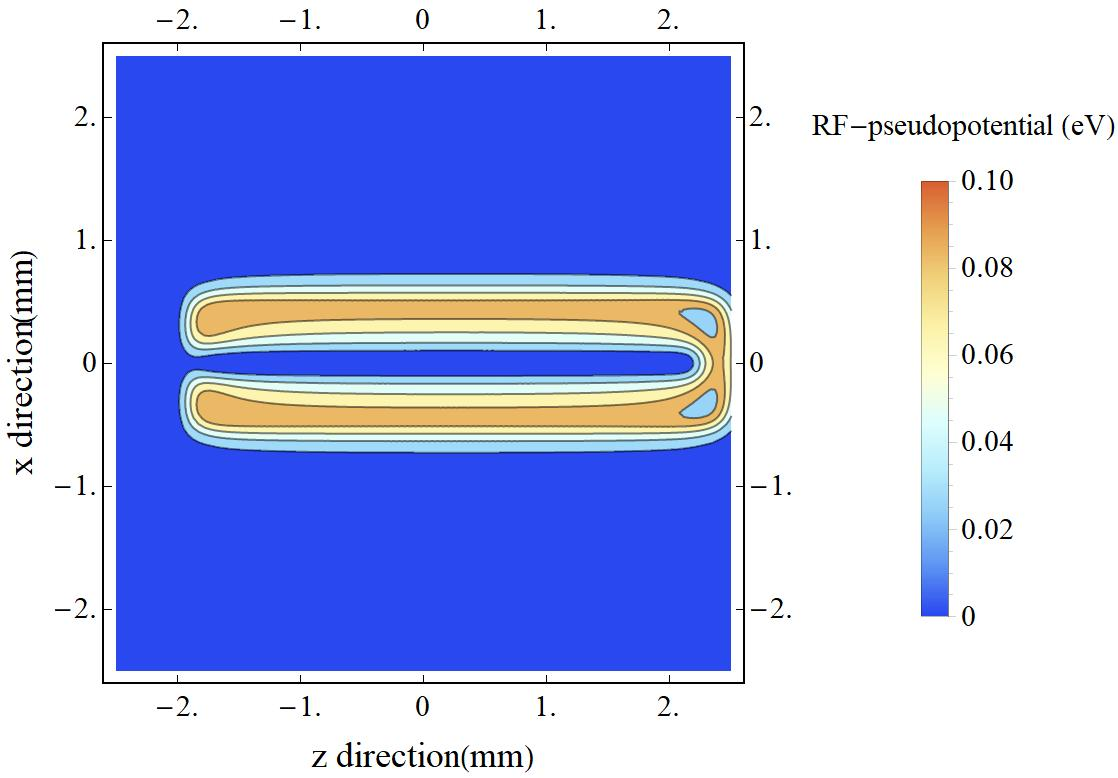
\includegraphics[width = 0.7\linewidth]{./simulation/figure/single-well_zx.jpg}
	\caption{z-x平面($y = 188.556 \ {\rm \mu m}$)でのSingle-wellにおけるrf擬ポテンシャル}
	\label{fig:single-well_example_zx}
	\end{center}
\end{figure}

\clearpage

\section{Double-wellにおけるrf擬ポテンシャル}
本実験で用いるプレーナートラップでは,rf電極に印加するrf電圧の振幅$V_{\rm rf}$とcenter-rf電極に印加するrf電圧の振幅$V_{\rm center-rf}$の比率
\large
\begin{align}
R = \frac{V_{\rm center-rf}}{V_{\rm rf}}
\end{align}
\normalsize
を制御することでイオンを二列に配列させることが可能になっている.

\Fig{R075}$\sim$\Fig{R100}に異なるRの値に対するrf擬ポテンシャルの変化の様子を示す.
\begin{figure}[h]
	\begin{minipage}{0.48\linewidth}
		\begin{center}
			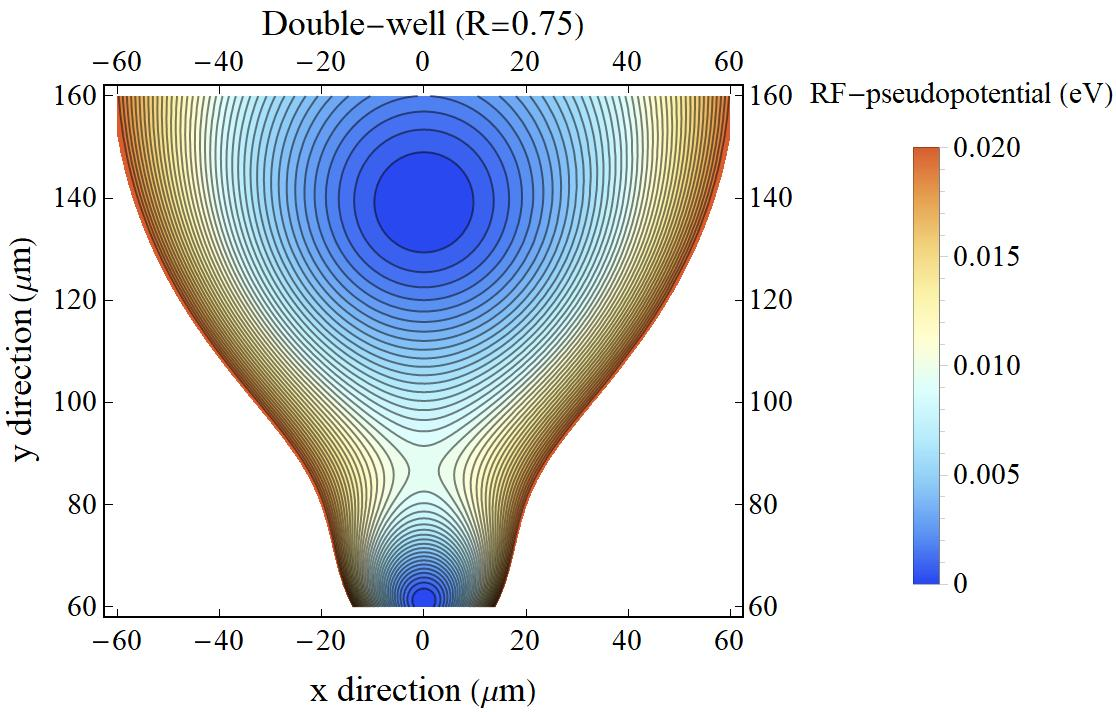
\includegraphics[width = 0.9\columnwidth]{./simulation/figure/rf_pseudopotential_R=075.jpg}
			\caption{$R=0.75$}
			\label{fig:R075}
		\end{center}
	\end{minipage}
	\begin{minipage}{0.48\linewidth}
			\begin{center}
				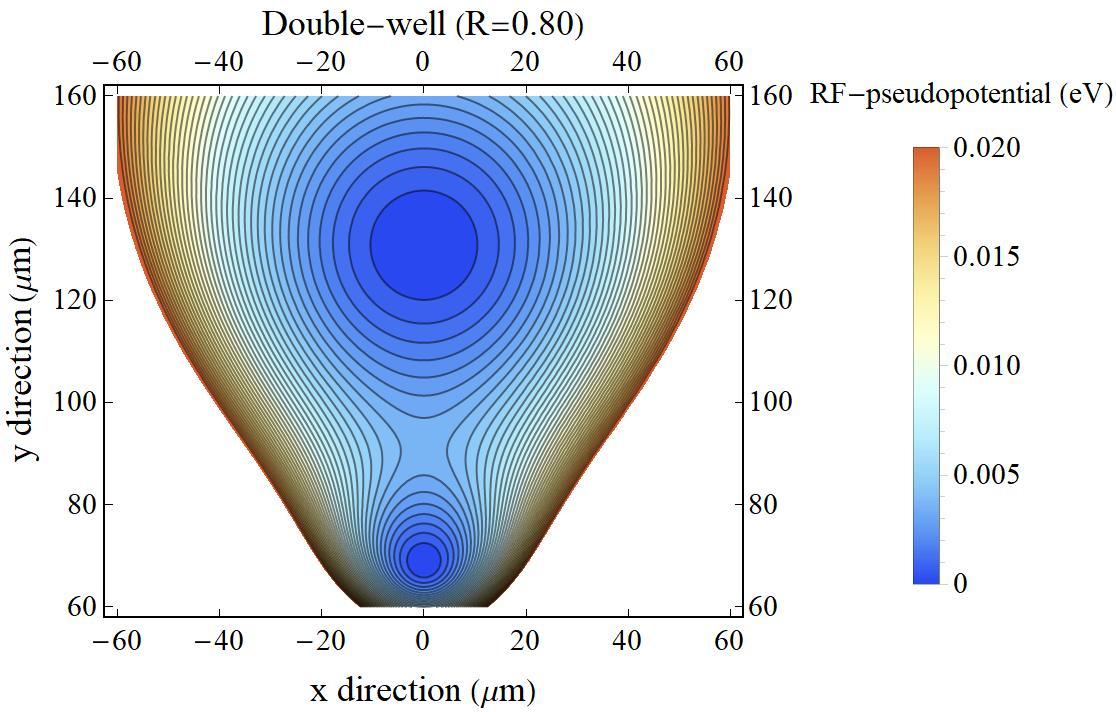
\includegraphics[width = 0.9\columnwidth]{./simulation/figure/rf_pseudopotential_R=080.jpg}
				\caption{$R=0.80$}
				\label{fig:R080}
			\end{center}
		\end{minipage}
\end{figure}
\begin{figure}[h]
	\begin{minipage}{0.48\linewidth}
		\begin{center}
			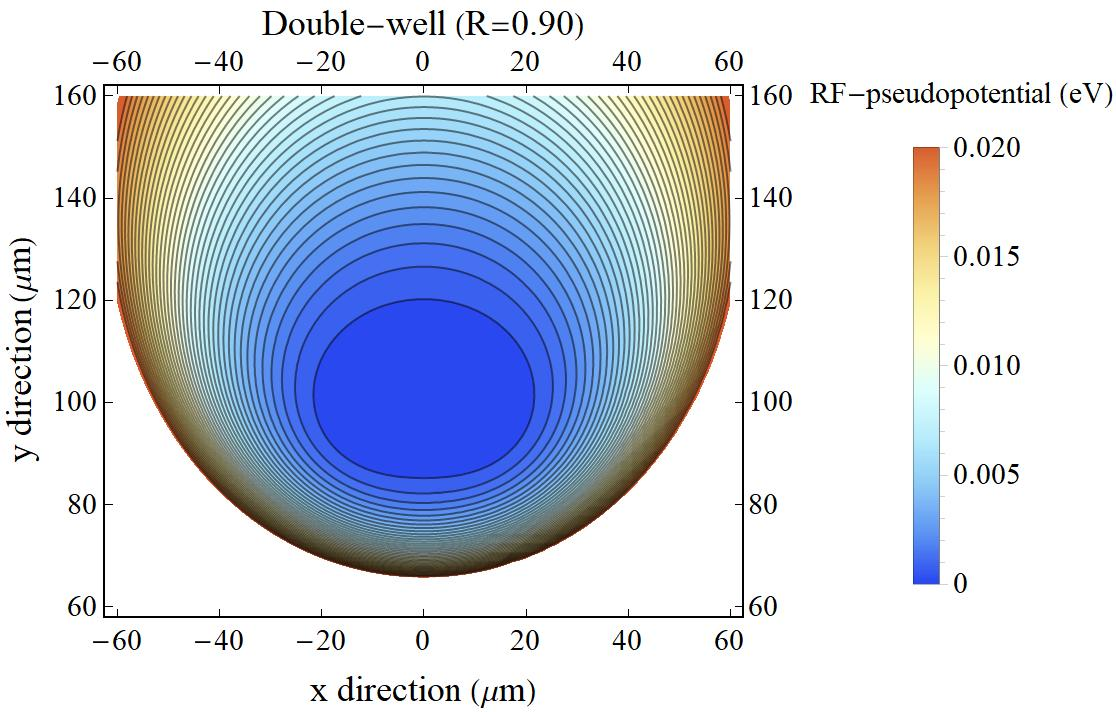
\includegraphics[width = 0.9\columnwidth]{./simulation/figure/rf_pseudopotential_R=090.jpg}
			\caption{$R=0.90$}
			\label{fig:R090}
		\end{center}
	\end{minipage}
	\begin{minipage}{0.48\linewidth}
			\begin{center}
				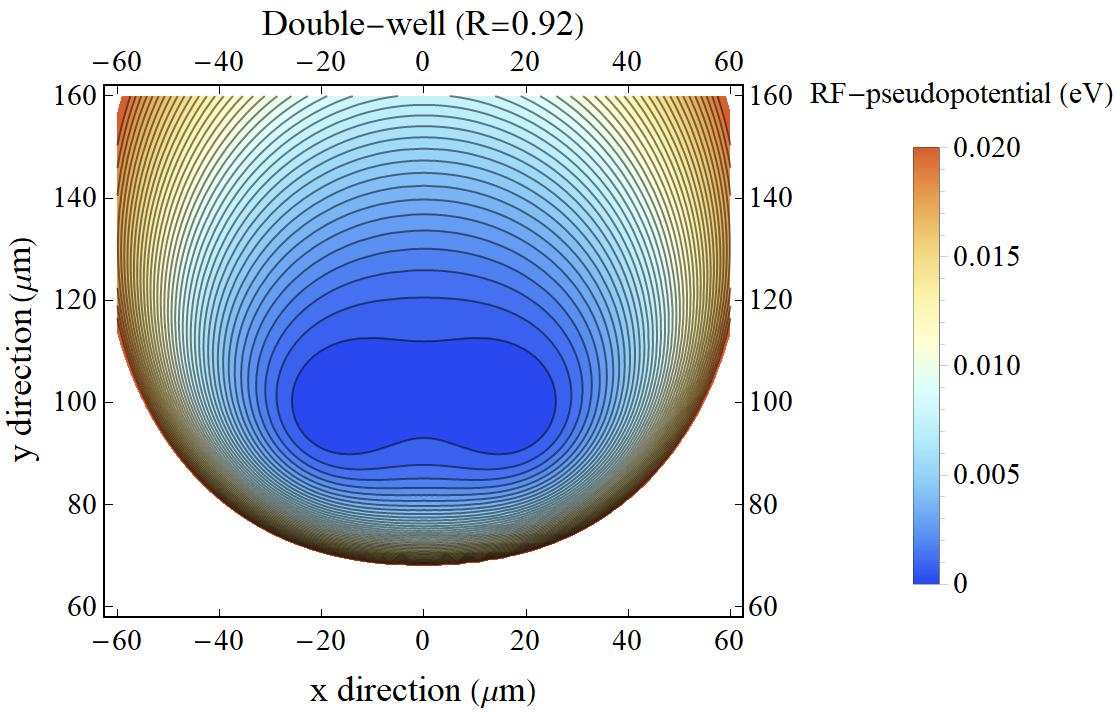
\includegraphics[width = 0.9\columnwidth]{./simulation/figure/rf_pseudopotential_R=092.jpg}
				\caption{$R=0.92$}
				\label{fig:R092}
			\end{center}
		\end{minipage}
\end{figure}
\begin{figure}[h]
	\begin{minipage}{0.48\linewidth}
		\begin{center}
			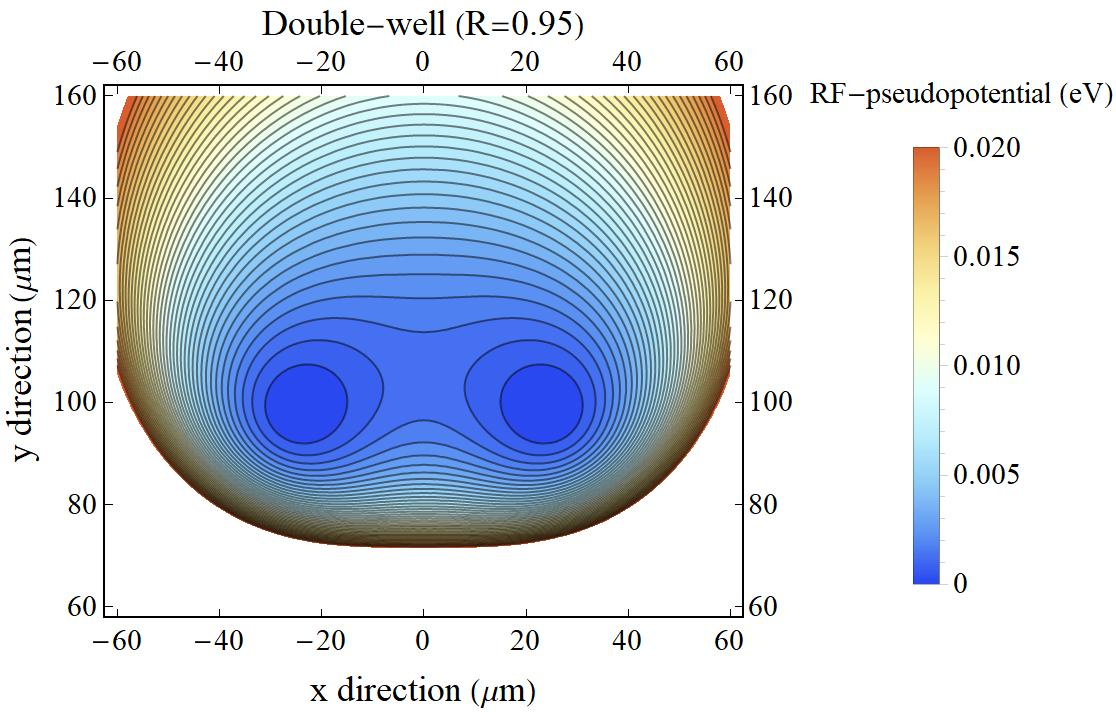
\includegraphics[width = 0.9\columnwidth]{./simulation/figure/rf_pseudopotential_R=095.jpg}
			\caption{R=0.95}
			\label{fig:R095}
		\end{center}
	\end{minipage}
	\begin{minipage}{0.48\linewidth}
			\begin{center}
				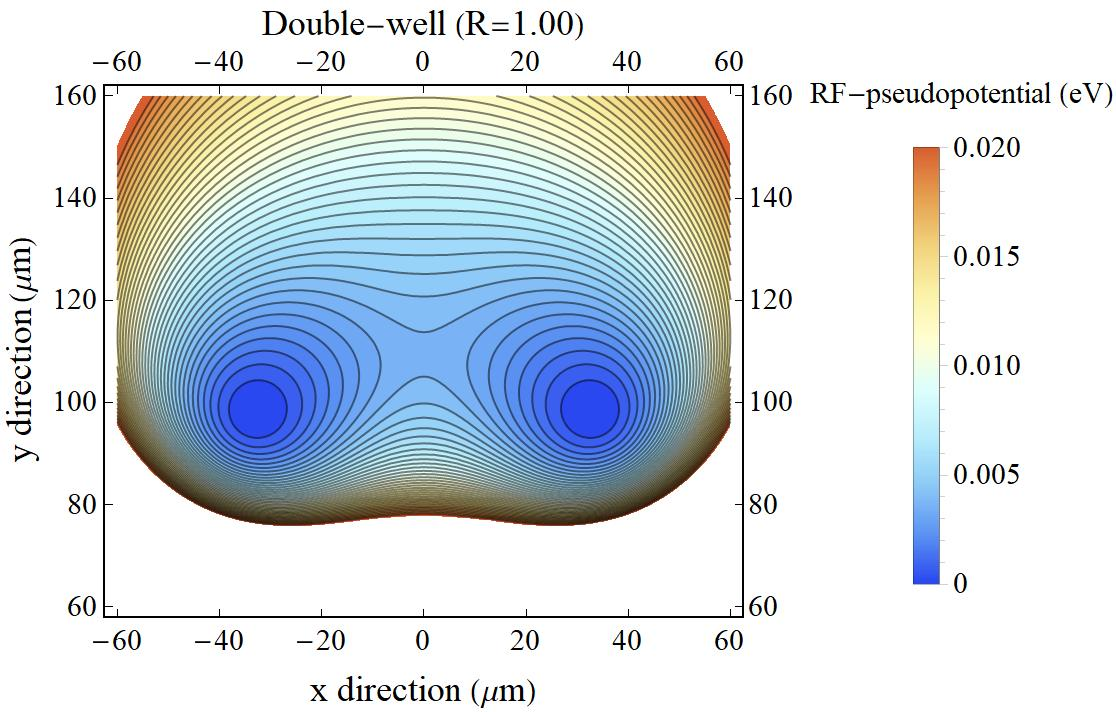
\includegraphics[width = 0.9\columnwidth]{./simulation/figure/rf_pseudopotential_R=100.jpg}
				\caption{$R=1.0$}
				\label{fig:R100}
			\end{center}
		\end{minipage}
\end{figure}

\clearpage

\section{Secularポテンシャル}
イオンを捕獲するときのトラップポテンシャルは,dcポテンシャルとrf擬ポテンシャルの重ね合わせ,
\large
\begin{align}
	\phi_{\rm secular} = \phi_{\rm DC} + \phi_{\rm eff}
\end{align}
\normalsize
で表される.これをSecularポテンシャルと呼ぶ.\Fig{SecPot_single-well}にその一例を示す.
\begin{figure}[h]
	\begin{center}
		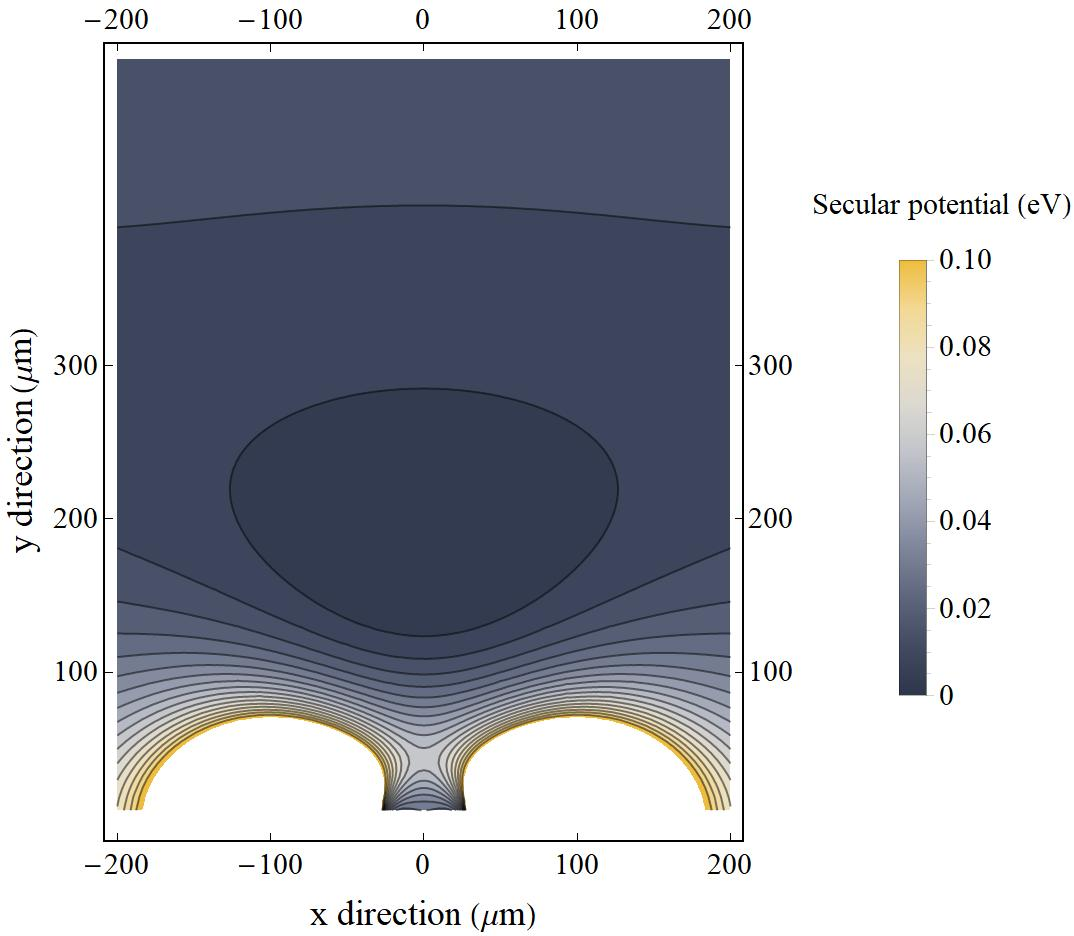
\includegraphics[width = 0.7\linewidth]{./simulation/figure/Secular_pot_xy.jpg}
		\caption{x-y平面でのSingle-wellの条件におけるSecularポテンシャル}
		\label{fig:SecPot_single-well}
	\end{center}
\end{figure}

\section{各方向における永年周波数}